\documentclass{article}
\usepackage[utf8]{inputenc}
\usepackage{blindtext}
\usepackage{enumitem}
\usepackage{graphicx}
\usepackage{hyperref}
\usepackage{titletoc}
\graphicspath{ {images/} }

\hypersetup{colorlinks=true,
urlcolor=blue,
linkcolor=black}

\title{ \begin{center}
					
\includegraphics[scale=0.6]{FEUPlogo}
				\end{center}
				\textbf{Werewolves of Miller's Hollow}}
\author{João Silva - up201405490\\
		Marcelo Ferreira - up201405323\\
		Miriam Gonçalves - up201403441}
\date{31 October, 2017}
\begin{document}

\maketitle

\thispagestyle{empty}

\newpage

\tableofcontents

\newpage

\section{Examination Paper}
\subsection{Scenario Description}
\textit{Werewolves of Miller’s Hollow} game is based on the russian game called “Mafia” and can be played by groups between eight and eighteen people. 
Game Components (24 roles):
\begin{center}
	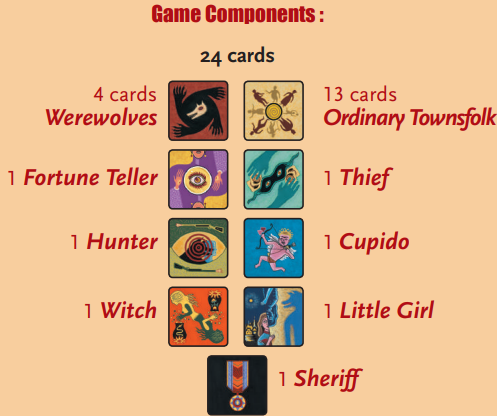
\includegraphics[scale=0.6]{gamecomponents}
\end{center}
	
\begin{itemize}
	\item \textbf{4 Werewolves}; 	
	\item \textbf{13 Ordinary Townsfolk} and there are 8 different kinds of Townsperson: 
	\begin{itemize}
		\item \textbf{1 Fortune Teller} - can see the true personality of one player each night, with its capacities it will help the townsfolk to find  correctly the identity of the werewolves;
		\item \textbf{1 Thief} - if this role is used, two additional ordinary Townsfolk are added at the beginning of the game. Afterwards two cards are placed face down in the center of the table, during the preliminary turn of the first night, this player looks at these two cards and may trade his/her cards with one of them. However if both of the cards are werewolves, the Thief must trade his card with one of them. If this player takes on of the extra cards, he/she assumes the role of this player for the rest of this character for the rest of the game;
		\item \textbf{1 Hunter} - if the hunter is killed during the game he can retaliate by eliminating another player;
		\item \textbf{1 Cupido} - got the ability to make any two people fall instantly in love for the rest of the game, these two people are designated during the first night of the game. If one of the lovers die, the other must kills him/herself immediatly. In case of one of the lovers being a townsperson and the other a werewolf, they must eliminate all the other players from the game to live in love and peace;
		\item \textbf{1 Witch} - make two kind of powerful potions: one is the \textit{healing} potion that can resurrect a player killed by a werewolf, the other is a \textit{poison} that kill a player during the night. Each potion can be used only once per game and use them on him/herself;
		\item \textbf{1 Little Girl} - this character can open her eyes during the night to spy on the werewolves, but if she gets caught by them she immediatly dies instead of the designated victim;
		\item \textbf{1 Sheriff} - this role is entrusted to one of the players, this person is elected by the townsfolk and once elected this player cannot refuse the honor. Afterwards this player's votes count as two votes. If this player dies during the game he/she must name his/her successor.
	\end{itemize}
\end{itemize}

For each number of players there are different combinations of roles:
\begin{center}
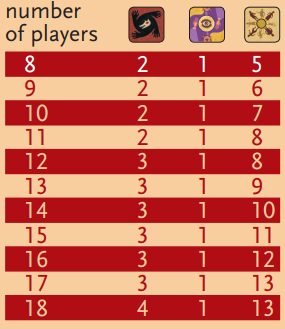
\includegraphics[scale=0.6]{playermix}
\end{center}

\setlength{\parindent}{0cm}There are two phases in the game: 
\begin{itemize}
	\item the night - when werewolves devour and kill one Townsperson (that person is eliminated from the game);
	\item the day - the townsfolk try to conceal their identity and discover who the werewolves are by voting on a suspect who is eliminated from the game.	
\end{itemize}

There are several points that players need to follow for setting up the game:
\begin{itemize}
	\item the players must choose a \textit{Moderator/Narrator}, this player must know very well all the games rules and create a strong atmosphere in order for the game to be fun;
	\item the \textit{Moderator} takes the appropriate number of cards, shuffles them and deals one character card to each player, from this step the players will look at their card secretly and places it face down in front of themselves;
	\item the \textit{Narrator} puts the town to sleep, all the characters must close their eyes.
	\item depending on the character cards on play the \textit{Narrator} will call one by one and in the following order \textit{The thief}, \textit{Cupido} and \textit{The Lovers} to play their roles.
\end{itemize}
After the setting up round, the \textit{Moderator} will call \textit{The Fortune Teller} to choose a player whose true personality she wants to know, after showing her the card she will fall asleep. Next the werewolves are called to designate silently a victim which will be revealed to every players the next morning when everyone is awake.
Right after the werewolves voting for killing a person, the \textit{Moderator} will call \textit{The Witch} to wake up, show her the victim chosen and asks her if she wants to use the healing or the poisoning potion. 
The next morning, every \textit{Townsperson} will wake up, know the character/s that was/were killed during the night and will try to unmask a \textit{werewolf} without letting anyone know their true identity by voting on one player that they think that is a \textit{Werewolf}, after being eliminated from the game this player will reveal his/her identity and will not be able to speak to the other players until the game ends, while the \textit{werewolves} will try to disguise themselves as ordinary Townsfolk and not be discovered by the other players.
The game will follow these steps repeatidly until the game ends.

The game ends when:
\begin{itemize}
	\item the townsfolk manage to eliminate all the werewolves;
	\item the werewolves kill the last townsperson;
	\item the lovers are the surviving townsperson/werewolf pair, and the all other players are dead; 
\end{itemize}

\subsection{Objectives}
This work has the goal to create the game \textit{Werewolves of Miller’s Hollow} following all the rules of the game, creating the different roles through different types of agents and evaluating their performance to see what agents are the most adequates for each role. 
\subsection{Expected results and evaluation form}

\section{Platform/Tool}
\subsection{JADE}
\subsubsection{What it is used for}
It simplifies the implementation of multi-agent systems through a middle-ware that complies with the FIPA specifications.
\subsubsection{Description of the main characteristics}
JADE is an opensource software fully implemented in JAVA. It allows to distribute agents across machines and the configuration can be controlled via a remote GUI. It also can be changed at run-time by moving agents to another machine. Each agent in JADE can have behaviours, that are tasks.
Another characteristics of JADE is the communication between agents.
\subsubsection{Highlight of the main features for the work}
For this work, JADE provides comunication peer-to-peer between agents.
\subsection{JASON}
\subsubsection{What it is used for}
JASON is a platform for the development of multi-agent systems. It is an interpreter for an extended version of AgentSpeak.
\subsubsection{Description of the main characteristics}
JASON is an opensource project and is developed in JAVA. It is fully customisable in JAVA, it can run a multi-agent system distributed over a network and implements the operational semantics of AgentSpeak.
\subsubsection{Highlight of the main features for the work}
For this work, JASON will be important to create BDI agents. 
\section{Specification}

\subsection{Agents}
In order for the game to take place, agents need to assume all the necessary parts. For our purposes we consider each role to be a different type of agent. As such, at the highest level of abstraction, there are two main roles: The players and the game coordinator.

Players are responsible to play the actual game. They must negotiate with other players, collaborate with their team and compete with the opposing team with the ultimate purpose of winning the game. How they go about achieving this is dependant on which role they play. In practice, character agents will be a subclass of the abstract player agent that implement their specific behaviors:

The game coordinator is responsible for controlling the flow of the game and relaying information about the environment to the players. It's the only purpose is to take the game all the way to completion.

\begin{center}
	\begin{tabular}{ p{3cm} l p{5cm} }
	Agent & Inherits & Description \\
	\hline
	Game Coordinator & N/A & Responsible for controlling the game flow\\
	Player & N/A \\
	Werewolf & Player & Plays the role of the werewolf \\
	Ordinary Townsperson & Player & Plays the role of the townsperson \\
	Fortune Teller & Player & Plays the role of the fortune teller \\
	Thief & Player & Plays the role of the thief \\
	Hunter & Player & Plays the role of the hunter \\
	Cupido & Player & Plays the role of the cupido \\
	Witch & Player & Plays the role of the witch \\
	Little Girl & Player & Plays the role of the little girl \\
	Sheriff & Player & Plays the role of the sheriff \\
	\end{tabular}
\end{center}

\subsection{Environment}
In order to formalize the agent's architecture let us first consider the environment in which the agents will live in. The game's environment is the game state in each round; the number of agents still in play and their roles. According to Russell and Norvig (Russell and Norvig, 2010, p.42), an environment can be either: Single-Agent or Multi-Agent; Fully Observable or Partially Observable; Deterministic or Non-deterministic; Episodic or Sequential; Static or Dynamic; Discrete or Continuous; and Known or Unknown. We'll address each of these in order.

The environment in which our agents interact is obviously multiagent, considering that the smallest number of agents required to play the game is eight. Not only that, it is a partially cooperative multiagent system given that agents on the same team (the townsfolk for example) must cooperate in order to win the game. But it is also a partially competitive multiagent system because, in the end, only one team is victorious; either the townsfolk kill all the werewolves, or the werewolves kill all the townsfolk.

Russell and Norvig describe a fully observable environment as an environment in which "the sensors detect all aspects that are relevant to the choice of action". That is decidedly not true in the environment of our game since agents purposely withhold information from each other. For example, a werewolf would not (except for strategic reasons) let others know that he is a werewolf, as that would get him lynched. As such the environment is partially observable; the agents cannot get reliable and up-to-date information regarding the environment from their sensors alone.

In a deterministic environment, the next state of the environment can be fully determined given only the current state and the action executed by the agent. Because of that, it is not obvious whether the environment of our game is deterministic or non-deterministic. In one hand there is uncertainty in the outcome of the actions of any agent; Say agent A decided that agent B is definitely a werewolf and votes to lynch them, but because the other agents do not agree with A, agent C is lynched instead. In this case, the agent action (vote to lynch B) resulted in B being lynched but had the other agents agreed with A then agent B would be lynched instead. It's then clear that the same action from an agent could result in more than one outcome, suggesting a non-deterministic environment. However, because the uncertainty arises purely from the actions of other agents a case can be made that the environment is actually deterministic in that the same actions from all the agents in the system will always result in the same outcome.

Deciding whether the environment is episodic or sequential is also not quite a trivial affair. At a glance we can say that each round is an episode, meaning that actions taken in each round are independent and do not depend on actions taken in previous rounds. But once we look closer it appears that that hypothesis does not hold; that some actions can have long-lasting consequences. For example, if the agents decide to kill the Fortune Teller early in the game, then from then on they have one less source of information from which to base their decisions on, affecting the way those decisions are made. The environment can then be considered sequential.

A somewhat easier property of the environment to identify is whether it is static or dynamic. In our game, the state of the environment does not change while an agent is deliberating. The game is played in turns, and every environment altering decision is made once at the end of each turn by all agents, making the environment static.

Discrete environments have a finite number of percepts and actions. This seems to be in line with the environment our game takes place in: The game is turn-based (or, in other words, is not a continuous-time problem) and there is only a finite number of states the environment can be in. 

The last property of the environment is related to the state of knowledge of an agent about the laws or rules of the environment. In the case of our game every agent is aware of the game's rules (otherwise they would have to learn as they played, which is very hard if not impossible given no base knowledge about the game) which means that the environment is known.

This makes our environment multiagent, partially observable, deterministic, sequential, static, discrete and known.

\subsection{Architecture}

The most appropriate architecture for the agents in our game is a BDI architecture. The reason for this is that there is very little information available about the environment in the beginning of the game; Each agent begin with just a few beliefs. Knowledge about the world is obtained through interactions with other agents but that information cannot be taken as a fact because agents may, intentionally or unintentionally, provide false information. That is what Beliefs are for; they portray the environment based on what a given agent believes it's true at any given point, but are subject to change whenever new information is gathered.

\subsection{Interaction Protocols}

Negotiation is central to our game, as it is mainly dialog based. More specifically agents will attempt to reach agreement through argumentation; In other words agents should try to persuade others to act in accord with their intentions. As such it is necessary to establish an argumentation scheme so that agents can generate and analyze arguments from their beliefs.

In each round of the game agents will go around to every other and try to convince them to act in accord to their own interests. In practice the negotiation will happen over the role of each agent in the game so that agents may choose who they want to see lynched.

Once an agent engages in negotiation with another one, then one (usually the initiatior) should assume the role of persuader and the other the role of the persuadee. Then in turns they present their arguments: the persuader tries to convince the persuadee to perform an action using some argument; then the persuadee either accepts or refuses, in which case it must provide a stronger argument. If the persuader wins the argument, then the persuadee changes its plans; otherwise everything stays the same.

It is then important to determine the types of arguments allowed. For our purposes we'll borrow the argument types proposed in "Reaching agreements through argumentation: a logical model and implementation" (Sarit Kraus, Katia Sycara, Amir Evenchik, 1998):
\begin{enumerate}
\item{Threats}
\item{Promise of future reward}
\item{Appeal to past promise}
\item{Counterexample}
\item{Appeal to self-interest}
\end{enumerate}

\subsubsection{Threats}
Threats can be used by a persuader to make a persuadee adopt one of the persuader's goals or to drop a goal that contradicts the its goals. 

Say agent $i$ tries asks agent $j$ to perform an action $\alpha$ but $j$ refuses on the grounds that $\alpha$ contradicts its goal $g_1$. Then $i$ could try to convince $j$ by threatening to perform $\beta$ that goes against a goal $g_2$ of $j$ (according to the beliefs of $i$). At that point $j$ should analyze the validity of the threat; Is $g_2$ more important to $j$ than $g_1$? Is $i$ cappable of carrying out its threat? If $j$ concludes that the threat is real then it could give in and perform $\alpha$ (abandoning its goal $g_1$).

\subsubsection{Promise of future reward}
An agent can entice another to perform an action that goes against its immediate goals by promising a reward, for example, performing an action that contributes to a goal that the former values highly. 

This is very much like trading favors; agent $i$ tries to get agent $j$ to perform $\alpha$ now by promising to perform $\beta$ in the future. In this situation $i$ may choose perform $\alpha$ if it decides that $\beta$ contributes to a goal that is highly valued.

\subsubsection{Appeal to past promise}
Promises are no good if agents do not keep them. As such, agents can appeal to promises that others have made to them and thus get them to act in accord with their goals.

It is important to note that agents can choose not to fulfill their promises. However, it may be in their best interest to do so, because if not other agents may label them as untrustworthy and promises of future reward arguments become ineffective.

\subsubsection{Counterexample}
If agent $j$ asks agent $i$ to perform action $\alpha$ and $i$ refuses on the grounds that $\alpha$ contradicts one of its goals $g_1$ then $j$ may inform $i$ that in the past $i$  performed action $\alpha$ and it did not condradict goal $g_1$. In other words, $j$ could try to convince $i$ using a counterexample.

\subsubsection{Appeal to self-interest}
At times an agent can decide that a certain action contributes to the goals of another agent, but that the latter is not aware of it, so it uses it as an argument to get him to perform it. This is called an appeal to self-interest.

\subsection{Project Plan}

The project must be constructed iteratively, with each iteration building on the previous one and resulting in a deliverable.

As such, we shall begin by implementing a simple game setup with just three types of agents: the Game Coordinator, the Townsperson, and the Werewolf. Also, at this point, the architecture will be fairly simple, not really involving negotiation and argumentation resulting in seemingly random agents.

Next, we will begin adding special characters, starting with the Fortune Teller. At the same time, we will improve the architecture and try to introduce negotiation even if not in the form of argumentation.

Following that, we will include all the other special characters and finalize the architecture so that it involves actual argumentation.

\section{Resources}

\subsection{Software}
JADE \par
\url{http://jade.tilab.com/} \par 
\vspace{3mm}
JASON \par
\url{http://jason.sourceforge.net/wp/} \par 

\subsection{Bibliography}
\noindent
(1) Wooldridge Michael, "An Introduction to MultiAgent Systems"

\noindent
(2) Ashraf El-Sisi, Hamdy Mousa, "Argumentation Based Negotiation in Multi-agent System"

\noindent
(3) Sarit Kraus, Katia Sycara, Amir Evenchik, "Reaching agreements through argumentation: a logical model and implementation"

\noindent
(4) Stuart Russell, Peter Norvig, "Artificial Intelligence: A Modern Approach"

\end{document}